
\documentclass[11pt]{article}


\usepackage[utf8x]{inputenc}
\usepackage{hyperref}
\usepackage{amsmath}
\usepackage{amssymb} 
\usepackage{textcomp}
\usepackage[francais]{babel}
\usepackage{natbib} 
\usepackage{hyperref} 


\usepackage{graphicx}
\graphicspath{ {./} }

\usepackage[top=0.8in, bottom=0.8in, left=0.8in, right=0.8in]{geometry}


\title{
   Le secret bancaire suisse au XXe siècle dans le
  \textit{Journal de Genève} et la \textit{Gazette de Lausanne}
}
\author{Yann Bolliger, Pietro Carta, Romain Mendez}

\begin{document}
\maketitle

\section{Contexte historique}

La place financière suisse a vu une énorme croissance presque non perturbée tout
au long du XXème siècle. Cela a été possible grâce à la neutralité et la
stabilité de la Suisse notamment en période de guerre mais surtout aussi grâce
au «secret bancaire»~\citep[p. 512]{Mazbouri12}. Ce dernier est déjà une
pratique des banques suisses au XIXème siècle quand les grandes
banques\footnote{Union de Banques Suisses, Schweizerische Kreditanstalt (Crédit
Suisse), Schweizerische Volksbank, Banque Leu, Eidgenössische Bank, Société de
Banque Suisse, Banque Commerciale de Bâle et le Comptoir d’Escompte} commencent
à dominer la place financière suisse. Ces banques-là profitent considérablement
des afflux de capitaux étrangers. Pendant la Grande Guerre les banques utilisent
le secret bancaire pour attirer les capitaux étrangers fuyant de lourdes
fiscalités implémentées par les pays en guerre~\citep[p. 484-486]{Mazbouri12}.
Cela permet aux banques de devenir une force majeur à l’échelle de la finance
mondiale ainsi qu’une influence principale dans la politique nationale.
En effet, l’influence des banques dans la politique fédérale est tellement
grande que le secret bancaire est renforcé par la loi sur les banques en 1934,
sans susciter de grands débats au parlement~\citep{Guex99}. 

L'introduction de cette loi est vue aujourd'hui comme la troisième étape de
l'avènement des paradis fiscaux contemporains~\citep[p. 29]{Chavagneux12}. La
première étape étant les états du Delaware et du New Jersey qui attirent des
entreprises avec des taxes très basses vers la fin du XVIIIème siècle. Une
décision des juges anglais de 1929 disant qu'une entreprise qui a son siège à
l'étranger n'est pas imposable en Angleterre a marqué la deuxième étape. Comme
ces deux étapes ont eu lieu dans des pays anglophones le terme anglais
\textit{tax haven} a été repris en français comme \textit{paradis fiscal}.

Avec la Seconde Guerre mondiale, de nouveau, la place financière Suisse profite
de la fuite de capitaux étrangers provenant de pays en guerre. Sous couvert de
la neutralité, les banques suisses arrivent à maintenir des liens très proches
avec tous les belligérants, mais surtout avec les forces de l’Axe, ce qui mène
la Suisse dans une grande isolation diplomatique à la fin de la guerre. Par
exemple, les États-unis gèlent les avoirs des banques suisses déposés en
Amérique déjà en 1941. Néanmoins la diplomatie suisse obtient le maintien du
secret bancaire contre les revendications des vainqueurs. Cela marque le début
d’une période de croissance sans précédent pour la place financière pendant les
«trente glorieuses»~\citep[p. 495]{Mazbouri12}.

Après la guerre, à l'étranger, le secret bancaire suisse reste objet de fortes
critiques. Les plus importants critiques étant les États-unis et la
France~\citep[p. 503]{Mazbouri12}. Dans la deuxième partie du XXe siècle, la
diplomatie américaine obtient de la Suisse quelques concessions qui ont
toutefois très peu d'impact. Après 1968, des critiques intérieures commencent a
troubler le consensus de la population suisse en faveur du secret bancaire. Au
même moment, de nombreux scandales impliquant les grandes banques Suisse font
surface. L’organisation tiers-mondiste “Déclaration de Berne” \citep{EvB} se
forme et dit lutter contre ``l'exploitation'' des pays en voie de développement
par le secteur financier et industriel suisse. Cette organisation lance,
conjointement avec le Parti Socialiste, une initiative populaire contre le
secret bancaire en 1984\footnote{Initiative populaire ``contre l'abus du secret
bancaire et de la puissance des banques''.
https://www.bk.admin.ch/ch/f/pore/va/19840520/index.html}. L'initiative
populaire est toutefois rejetée par une forte majorité des suisse (73\%).

Avec l'accord du peuple, les grandes banques ont ainsi maintenu le
statut privilégié de la place financière pendant plus que 50 ans. Ils l’ont
défendu contre la pression de l’intérieur et de l’extérieur. Ce n’est
seulement après la crise financière en 2007 que, sous la pression de l'OCDE,
le secret bancaire est aboli pour les citoyens de pays membres de l'OCDE 
sauf la Suisse \citep{NeufVies}.
Il est à noter que des lois similaires existaient dans d'autres pays européens
qui ont tous graduellement cédé sous la pression des critiques. Pour beaucoup
c'est via la construction européenne que leurs lois sont influencées pour 
limiter le secret bancaire \citep[p. 32]{Palan09}. 

Dans le cadre de notre recherche nous essayerons de retrouver ces événements
dans la presse romande. Celle-ci étant plutôt proche des cercles financiers –
surtout le «journal de Genève» \citep{ConfClass1} –, nous évaluerons aussi
leurs positions sur le secret bancaire et si cette proximité peut-être
confirmée par les articles du corpus. Afin de nous demander, comment évolue la
couverture médiatique du secret bancaire au XXe siècle ? 

\section{Information Bibliographiques}
\subsection{Sources primaires}

Nous admettons dans notre analyse les articles extrait de la \textit{Gazette de
Lausanne} et du \textit{Journal de Genève}, pendant la
période 1900-1995. Pour restreindre l’analyse aux articles pertinents, le corpus
d’articles des deux journaux sera filtré en ne gardant que les articles
contenant des mots clés, repérés à travers l’analyse de nos autres sources
primaires et la littérature secondaire.

Les sources primaires que nous analysons, outres que les archives du Temps, sont
de nature politique, juridique, ou diplomatique. La “Déclaration de Berne” en
collaboration avec le Parti Socialiste publie en 1978 le pamphlet “Les Secrets
du secret bancaire suisse” \citep{GiovanniniPierLuigi1978Lsds} où les
conséquences internationales et intérieures du secret bancaire sont dénoncées.
Cet ouvrage nous expose au débat qui entourait le sujet pendant les années 70 et
80.

Les sources juridiques témoignent d'un conflit entre la Suisse et des pays
étrangers dans le domaine du secret bancaire. Les Americains étudient déja en
1969 les aspects juridiques du secret bancaire \citep{Mueller69}. Ce qui mène à
un procès auprès du tribunal fédéral \citep{tribunalFederal70}, qui se conclut
en 1970 en faveur du maintien du secret bancaire. Nous étudierons aussi l'accord
bilatéral entre la Suisse et les Etats-Unis sur le secret bancaire, comme
témoigné dans un rapport du \citet{insiderTrading83}.

\subsection{Littérature secondaire}

Nous considérons deux types de littérature secondaire, un sur l’histoire financière
suisse par Sébastien Guex et Malik Mazbouri \citep{Guex99, Guex00, Mazbouri12}.
Et un autre type sur les spécificités du cas suisse au niveau international,
analysé par Henry Meier \citep{Meier12}.

\subsection{Mots-clés}

Notre corpus consistant de milliers d'articles différents, il est nécessaire
d'isoler des mots-clés caractérisant notre sujet. C'est avec les termes
ci-dessous que nous trouvons le plus d'articles en lien avec le sujet.

Secret bancaire, place financière suisse, banques suisses, forfait fiscal,
paradis fiscal, corruption, affaire Chiasso, argent sale, blanchiment, PIB,
emploi, croissance.



\section{Outils Méthodologiques}

Afin de pouvoir traiter en un temps raisonnable notre corpus de texte, plusieurs
pistes d’analyse s’offrent à nous. Dans un premier temps un filtrage des
articles s’impose, pour ne travailler que sur des articles contenant des termes
importants du sujet (voir la liste de terme clés dans la précédente partie).
Aussi, nous pouvons lier l'apparition du terme secret bancaire à des événements
liés au sujet et voir l'évolution de la popularité du terme au fil du temps
comme dans la figure 1.

\begin{figure}[!htb]
  \centering
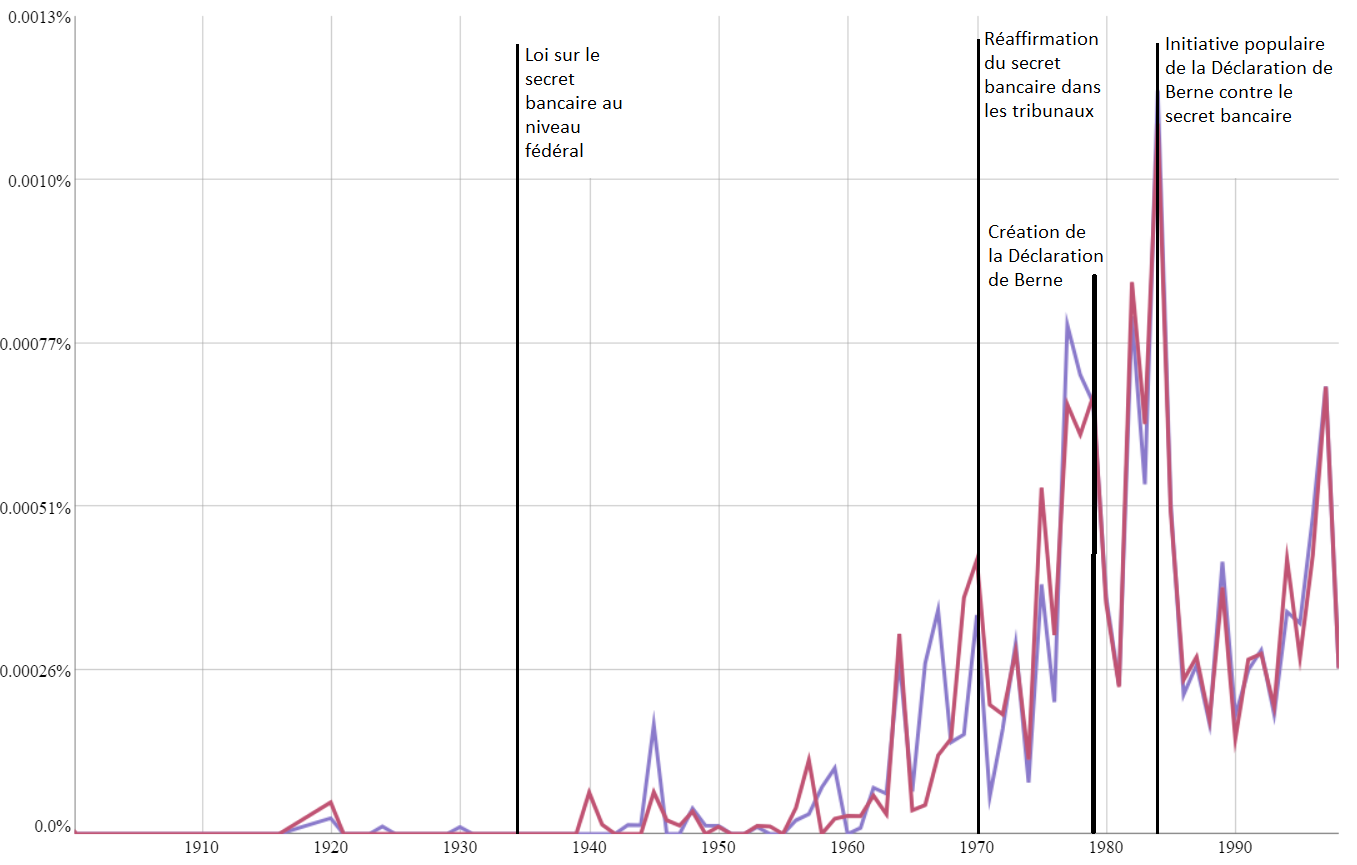
\includegraphics[width=0.8\textwidth]{ngram.png}
\caption{
  N-gram du terme "secret bancaire" dans les journaux \textit{Journal de Genève}
  (bleu) et \textit{Gazette de Lausanne} (rouge).
}
\end{figure}

\begin{figure}[!htb]
  \centering
  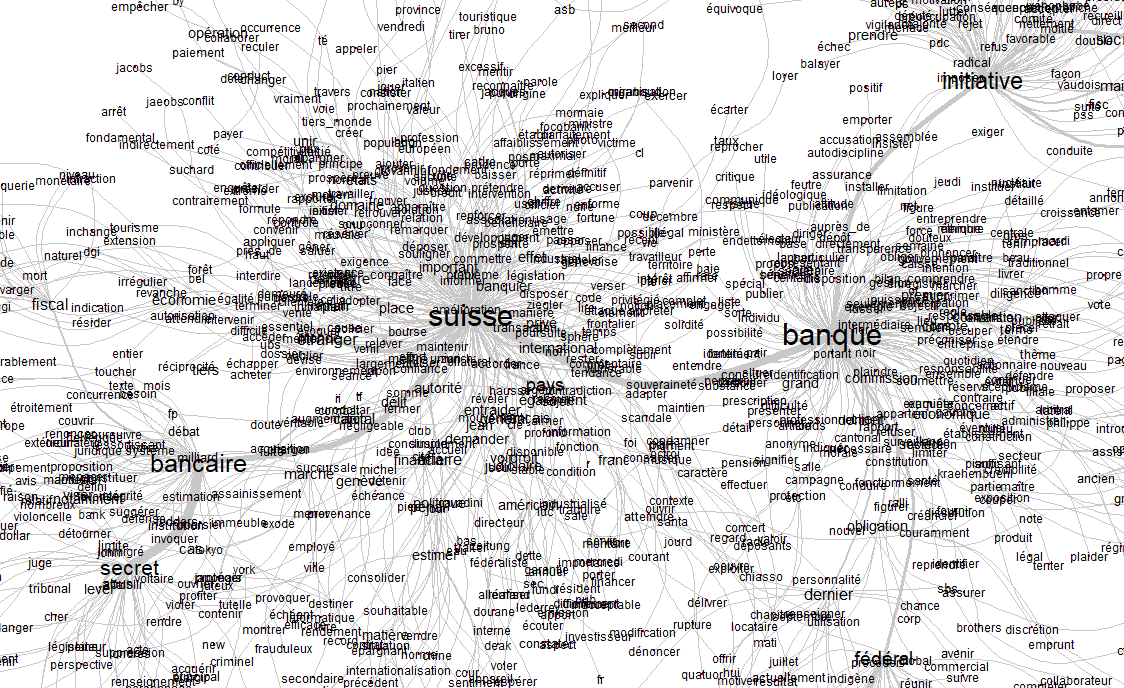
\includegraphics[width=1.0\textwidth]{reduced.png}
  \caption{Zoom dans la visualisation sur les articles contenant les mots "secret 
bancaire" dans l'année 1984 dans le \textit{Journal de Genève}}
\end{figure}

Ensuite, nous pensons procéder à des visualisations du corpus filtré avec des
logiciels tel que Iramuteq afin de voir les relations entre les mots (quels mots
se suivent souvent, et quelle est leur connotation).

Avec de telles visualisation nous voulons trouver plus de mots-clés. Par exemple
dans la figure 2, nous pouvons voir que les mots "secret" et "bancaire" sont peu
liés aux mots "initiative" et "populaire" en 1984 (alors qu'une initiative
populaire sur le sujet du secret bancaire est lancée cette année là). Ici on
peut voir que les thèmes en question sont toujours liés à la Suisse en
elle-même. Dans les mots autour de "initiative" on peut trouver d'autres mots
forts comme "balayer" ou "socialiste", ce qui indique par exemple une certaine
position dans les articles parlant de l'initiative.

Nous voulons tenter de répondre aux questions suivantes : A qui est-ce que la
parole est-elle donnée dans les journaux ? Est-ce que les acteurs étrangers
s'expriment ? Et surtout, est-ce que les banques sont promues ?

Cette dernière question nous amène à nous demander, comment détecter si les
banques sont promues et/ou critiquées ? L'idée actuelle est de voir si des
mots-clés traditionnellement associés au point de vu positif sont dans les
articles abordant le sujet ou non (tel que PIB, emploi, croissance ...).
    
Nous pensons donc utiliser les sources secondaires pour forger une attente du
corpus, ce à quoi nous nous attendons après ce type d’analyse. C’est-à-dire par
exemple utiliser les informations recueillies sur les rédactions des journaux
dans la conférence du 31 Octobre \citep{ConfClass1} afin de vérifier nos
résultats avec les différentes tendances des rédactions de ces deux journaux.
Cela devrait pouvoir nous servir de garde-fou sur nos résultats. Une fois ce
travail accompli, nous nous servirons des résultats pour analyser la position
idéologique des journaux au fil de la période étudiée. 

\newpage

\bibliographystyle{agsm}
\bibliography{bib/bibliography}

\end{document}
